\section{L04-Sistemi bifase}
\subsection{Sistema eterogeneo}
Un sistema \textbf{omogeneo} è un sistema con un solo stato di aggregazione.\newline
\newline
Un sistema \textbf{eterogeneo} è un sistema con più stati di aggregazione.\newline
\newline
Un sistema \textbf{monocomponente} è un sistema con una sola sostanza al suo interno.\newline
\newline
Un sisteam \textbf{multicomponente} è un sistea con più sostanze al suo interno.\newline
\newline
Le generica \textbf{grandezze estensive specifiche} $e$ di un sistema eterogeneo costituito da due stati di aggregazione $\alpha$ e $\beta$ possono essere rappresentate come \textbf{media pesata sulle masse} dei valori delle grandezze estensive specifiche delle singole fasi:
\[
    e = \frac{M_\alpha}{M}e_{\alpha} + \frac{M_\beta}{M}e_\beta
\]
\ \newline
Si definisce \textbf{frazione massica} le proporzioni di massa in uno stato di aggregazione rispetto alla massa complessiva. Per esempio in un generico sistema eterogeneo con due stati di aggregazione $\alpha$ e $\beta$:
\[
    x_\alpha = \frac{M_\alpha}{M} \;\;\;\;\;\;\;\;\;\;\;\;\;\;\; x_\beta = \frac{M_\beta}{M}
\]
Ricordiamo inoltre che 
\[
    x_\alpha + x_\beta = 1
\]
e che una generica grandezza estensiva specifica può quindi essere espressa come
\[
    e = x_\alpha e_\alpha + x_\beta e_\beta = (1-x_\beta)e_\alpha + x_\beta e_\beta
\]
\subsubsection{Regola di gibs per sistemi eterogenei}
\textbf{Regola di Gibbs}:
\[
    V = C + 2 -F
\]
$V$: numero di \textbf{variabili intensive indipendenti} utilizzabili per descrivere il generico stato di equilibrio.\newline
$C$: numero di componenti.\newline
$F$: numero di fasi.
\begin{itemize}
    \item Per il generico sistema \textbf{monocomponente e monofase} $V =2$, quindi per descrivere uno stato di equilibrio è sufficiente una coppia intensiva-intensiva (per esempio $P$ e $T$).
    \item Per il generico sistema \textbf{monocomponente bifase} $V =1$, quindi per descrivere lo stato termodinamico è necessaria una coppia intensiva-estensiva oppure un coppia estensiva-estensiva:\newline
    $(P,v) \;\; (T,v) \;\; (P,u) \;\; (T,u) \;\; (P,h) \;\; (T,h) \;\; (P,s) \;\; (T,s) \;\; (v,u) \;\; (v,h) \;\; (v,s) \;\; (u,h) \;\; (u,s) \;\; (h,s)$
    \item Per il generico sistema \textbf{monocomponente trifase} $V=0$, quindi per descirvere uno stato di equilibrio è necessaria un coppia estensiva-estensiva:\newline
    $(v,u) \;\; (v,h) \;\; (v,s) \;\; (u,h) \;\; (u,s) \;\; (h,s)$
\end{itemize}
\subsubsection{Transizione di fase}
Una \textbf{transizione di fase}:
\begin{itemize}
    \item è il passaggio da uno stato di aggregazione ad un altro;
    \item avviene a pressione (e temperatura) costatne.
\end{itemize}
\ \newline
Definiamo l'\textbf{entalpia di transizione} come la quantità di energia necessaria per passare da uno stato a un altro:
\[
    dh = \delta q^\leftarrow 
\]
\subsubsection{Sistemi eterogenei monocomponente}
Possibili configurazioni:
\begin{itemize}
    \item \textbf{Stati monofase}:
    \begin{itemize}
        \item Solido
        \item Liquido 
        \item Aeriforme (Gas)
    \end{itemize}
    \item \textbf{Stati bifase}:
    \begin{itemize}
        \item Coesistenza di solido e liquido
        \item Coesistenza di solido e aeriforme (vapore)
        \item Coesistenza di liquido e aeriforme (vapore)
    \end{itemize}
    \item \textbf{Stati tripli}:
    \begin{itemize}
        \item Coesistenza di solido, liquido e aeriforme (vapore)
    \end{itemize}
\end{itemize}
Terminologia:
\begin{itemize}
    \item \textbf{Liquido sottoraffreddato}: liquido non in porcinto di evaporare (temperatura di sistema sotto temperatura di saturazione)
    \item \textbf{Liquido saturo}: liquido in procinto di evaporare (liquido a temperatura di saturazione)
    \item \textbf{Vapore saturo}: vapore in condizioni di incipiente condensazione (gas a temperatura di saturazione)
    \item \textbf{Vapore surriscaldato}: vapore non in procinto di condensare (temperatura di sistema sopra temperatura di saturazione)
    \item \textbf{Temperatura di saturazione}: temperatura alla quale una sostanza pura comincia ad evaporare (se è un liquido) oppure condensare (se è un gas), fissata la pressione.
\end{itemize}
\subsection{Diagramma di stato P-v-T}
\subsubsection{terminologia}
\begin{center}
    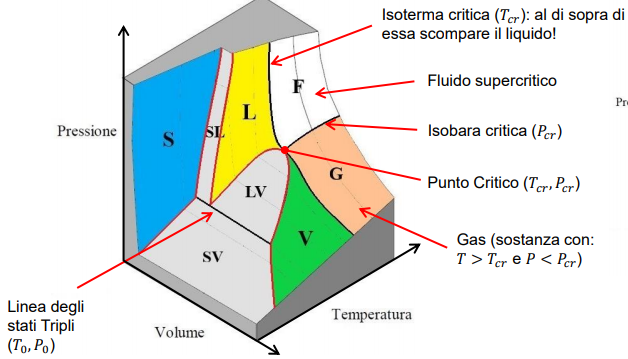
\includegraphics[height=5cm]{../L04/img2.PNG}
\end{center}
\begin{center}
    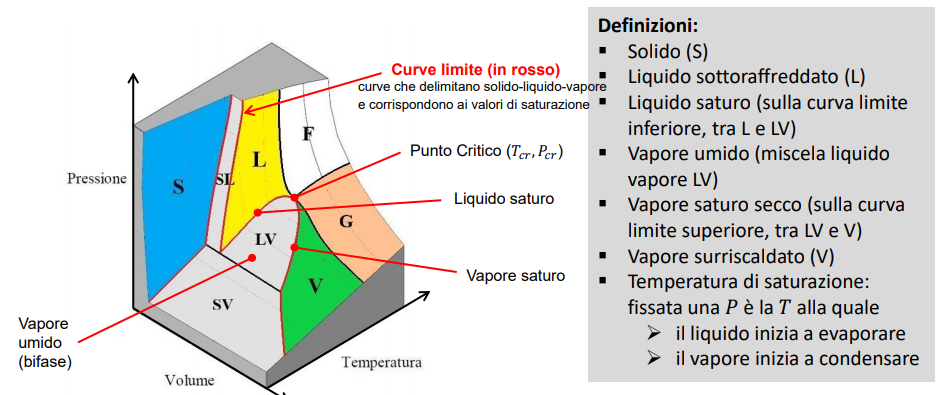
\includegraphics[height=5cm]{../L04/img1.PNG}
\end{center}
\subsubsection{Proiezione del diagramma P-v-T in un grafico P-T}
\begin{center}
    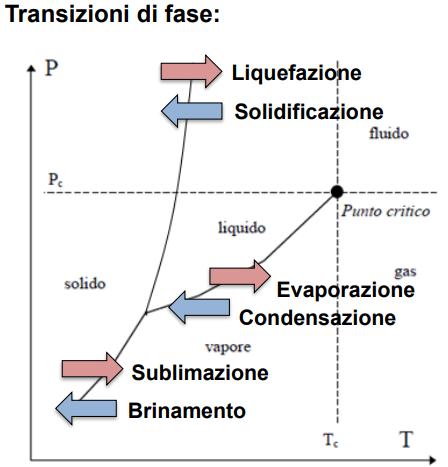
\includegraphics[height=7cm]{../L04/img3.PNG}
\end{center}
\subsubsection{Gas}
Fluido a $P< P_{cr}$ e $T> T_{cr}$ che non può essere liquefatto attraverso una trasformazione di compressione isoterma:
\begin{center}
    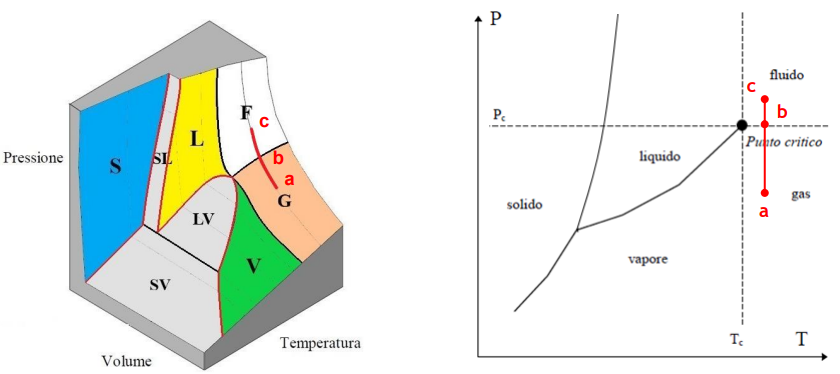
\includegraphics[height=7cm]{../L04/img4.PNG}
\end{center}
\subsubsection{Trasformazione isobara}
\begin{center}
    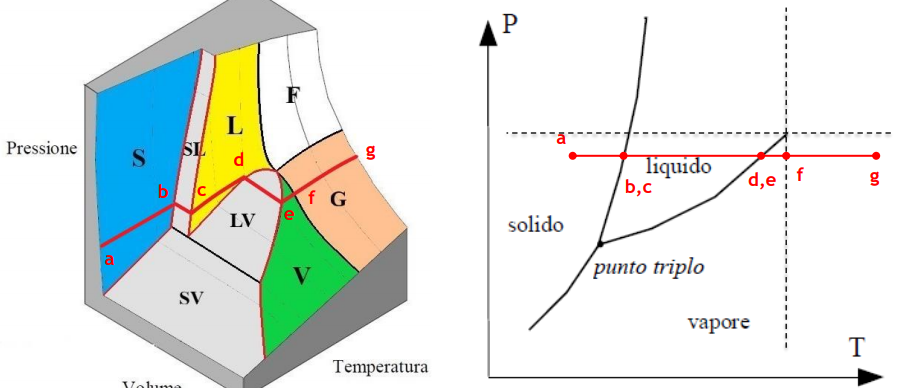
\includegraphics[height=6cm]{../L04/img6.PNG}
\end{center}
\begin{center}
    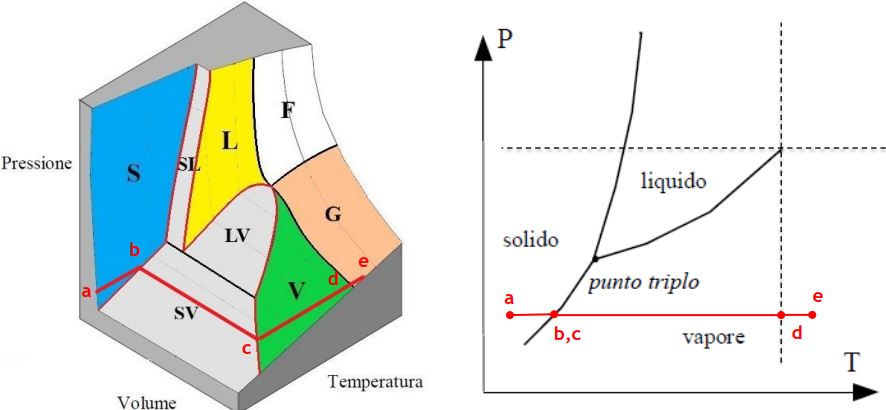
\includegraphics[height=7cm]{../L04/img5.PNG}
\end{center}
\subsubsection{Traformazione isoterma}
\begin{center}
    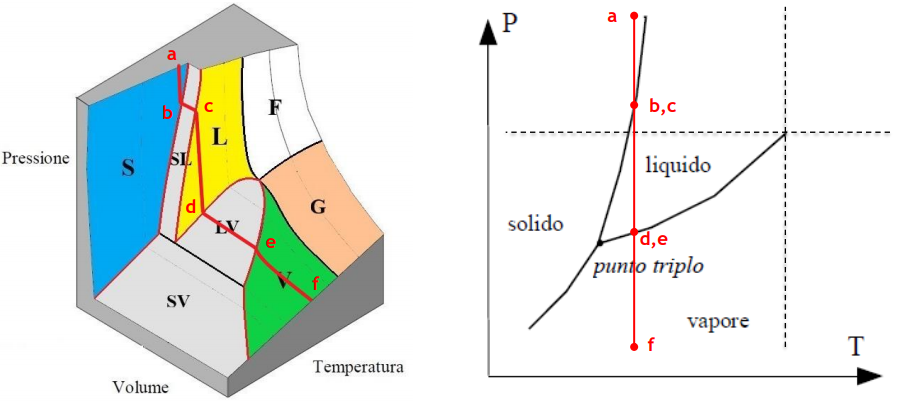
\includegraphics[height=6cm]{../L04/img7.PNG}
\end{center}
\subsubsection{Proiezione del diagramma P-v-T in un grafico P-s e P-h}
Uno dei problemi del proiettare la superficie di stato ne ldiagramm $P-T$, è che difficilmente riusciamo a rappresentare le transizioni di fase, perchè, per esempio le zone SL e LV corrispondono soltanto a un punto. Perciò il diagramma $P-T$ è poco utili per rappresentare i cambi di stato. Per ovviare a ciò dobbiamo fare diverse proiezioni della superficie di stato, rispetto a una coppia di grandezze $(P,v)$, per esempio:
\begin{center}
    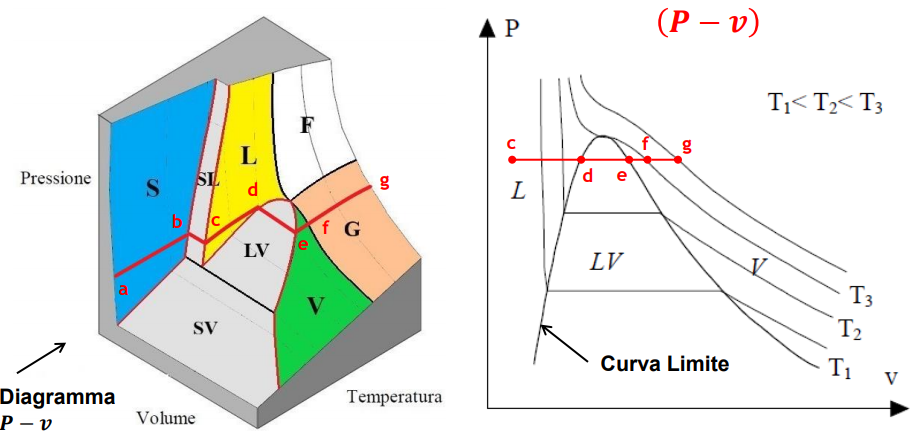
\includegraphics[height=6cm]{../L04/img8.PNG}
\end{center}
Una soluzione a questo problema di rappresentazion è l'utilizzo del diagramma temperatura-entropia, per esempio:
\begin{center}
    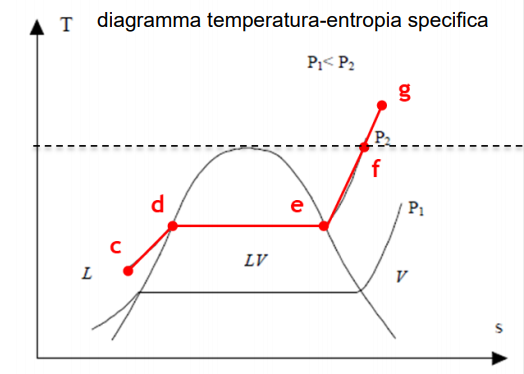
\includegraphics[height=6cm]{../L04/img9.PNG}
\end{center}
Il tipo di diagramma utilizzato varia a seconda dello scopo che si vuole raggiungere, ce ne sono anche molti altri, per esempio quello $P-h$ e quello $h-s$.
\subsection{Proprietà termodinamiche dei sistemi eterogenei}